\documentclass[apj]{emulateapj}

%Specify packages
\usepackage{amsmath}
\usepackage{tikz}
\usetikzlibrary{shapes.geometric, arrows}
\usepackage[tight]{subfigure}
\usepackage[breaklinks,colorlinks,citecolor=blue]{hyperref}
\usepackage[all]{hypcap}
\usepackage[utf8]{inputenc} %force unicode in bibtex
\usepackage{enumitem}
%use for editing/highlighting
\usepackage{color,soul}
%\usepackage{lineno}


%Define new commands as needed
\newcommand{\ang}{\AA~}
\defcitealias{barnes_inference_2016}{Paper I}
\renewcommand{\sectionautorefname}{Section}
\renewcommand{\subsectionautorefname}{Subsection}
%\linenumbers
%Set options for list spacing
\setenumerate{noitemsep}
%Set tikz options
\tikzstyle{box} = [rectangle, rounded corners, text centered, draw=black]
\tikzstyle{ghost} = [rectangle, rounded corners, text centered, draw=white]
\tikzstyle{arrow} = [thick, ->, >=stealth]

\begin{document}
	%Frontmatter
	\title{Inference of Heating Properties from ``Hot'' Non-flaring Plasmas in Active Region Cores II. Nanoflare Trains}
	\shorttitle{``Hot'' Non-flaring Plasmas II. Nanoflare Trains}
	\author{W. T. Barnes}
	\affil{Department of Physics \& Astronomy, Rice University, Houston, TX 77251-1892}
	\email{will.t.barnes@rice.edu}
	\author{P. J. Cargill}
	\affil{Space and Atmospheric Physics, The Blackett Laboratory, Imperial College, London SW7 2BW}
	\affil{School of Mathematics and Statistics, University of St. Andrews, St. Andrews, Scotland KY16 9SS}
	\and
	\author{S. J. Bradshaw}
	\affil{Department of Physics \& Astronomy, Rice University, Houston, TX 77251-1892}
	%Abstract
	\begin{abstract}
		Faint, high-temperature emission in active region cores has long been predicted as a signature of nanoflare heating. However, the detection of such emission has proved difficult due to a combination of the efficiency of thermal conduction, non-equilibrium ionization, and inadequate instrument sensitivity. In this second paper in our series on ``hot'' non-flaring plasma in active regions, we investigate the influence of repeating nanoflares of varying frequency on the resulting emission measure di . We have used an efficient two-fluid hydrodynamic model to carry out a parameter exploration in preferentially heated species, heating event frequency, and the power-law index determining the distribution of event energies. By computing the emission measure distributions and calculating their ``hotward'' slopes, we have concluded that not treating the electron and ion populations separately leads to a mischaracterization of the hot emission. Additionally, we find that, while emission due to separate electron and ion heating differs greatly hotward of the peak, the respective coolward emission measure slopes are similar such that a distinction between the heating of one species over another based on this criteria alone is not possible. 
	\end{abstract}
	%Body
	\section{Introduction}
	\label{sec:intro}
	%
	\par Heating of the solar corona by nanoflares, first proposed by \citet{parker_nanoflares_1988}, has become one of the most favored and contentious coronal heating models  \citep{cargill_implications_1994,cargill_nanoflare_2004,klimchuk_solving_2006}. The term \textit{nanoflare} has now become synonomous with impulsive heating in the energy range $10^{24}-10^{27}$ erg, with no specific assumption regarding the underlying physical mechanism; though its origin is almost certainly magnetic.
	%
	\par \citet{cargill_implications_1994,cargill_nanoflare_2004} have predicted that emission measure distributions resulting from nanoflare models should be wide and have a faint, high-temperature (8-10 MK) component, the so-called ``smoking gun'' of nanoflare heating. Though many workers \citep{reale_evidence_2009,schmelz_hinode_2009,miceli_x-ray_2012,testa_hinode/eis_2012,del_zanna_elemental_2014,petralia_thermal_2014,schmelz_hot_2015} have claimed evidence of this hot, faint component of the emission measure, poor spectral resolution \citep{testa_temperature_2011,winebarger_defining_2012} and non-equilibrium ionization \citep{bradshaw_explosive_2006,reale_nonequilibrium_2008} have made a positive detection of nanoflare heating difficult. However, \citet{brosius_pervasive_2014}, using obsservations from the \textit{EUNIS-13} sounding rocket, identified relatively faint emission from Fe XIX in a non-flaring active region (AR), suggesting temperatures of $\sim8.9$ MK.
	%
	\par One strategy for constraining potential heating models is analysis of modeled and observed emission measure distributions in active region (AR) cores. Originally proposed by \citet{jordan_structure_1975}, it is well-known that the emission measure, $\mathrm{EM}(T)=\int n^2\mathrm{d}h$, scales as $\mathrm{EM}(T)\sim T^a$ over a temperature range $10^6\lesssim T\lesssim T_m$, where $T_m$ is the temperature at which $\mathrm{EM}(T)$ peaks. Observations have shown that $2\lesssim a\lesssim5$, with $T_m\approx10^{6.5-6.6}$ \citep{warren_constraints_2011,warren_systematic_2012,winebarger_using_2011,tripathi_emission_2011,schmelz_cold_2012,del_zanna_evolution_2015}. 
	%
	\par A similar scaling has been claimed for hot emission such that $\mathrm{EM}\propto T^{-b}$. Typically, this power-law fit to the emission measure is done ``hotward'' of the peak, usually in the range $T_m\lesssim\log{T}\lesssim7.2$. However, measured values of these hotward slopes are poorly constrained due to both the magnitude of emission and the lack of available spectroscopic data in this temperature range \citep{winebarger_defining_2012}. \citet{warren_systematic_2012}, find $7\lesssim b\lesssim10$, with uncertainties of $\pm2.5-3$, for 15 AR cores thoguh \citet{del_zanna_elemental_2014}, using observations from the Solar Maximum Mission, claim larger values for $b$.
	%
	\par An important parameter for any proposed coronal heating mechanism is the frequency of energy release. Nanoflare heating is often classified as either \textit{high-frequency} or \textit{low-frequency} heating. In the case of high-frequency heating, $\langle t_N\rangle$, the time between successive events, is such that $\langle t_N\rangle\ll\tau_{cool}$, where $\tau_{cool}$ is the loop cooling time, and in the case of low-frequency heating $\langle t_N\rangle\gg\tau_{cool}$ \citep{cargill_modelling_2015}. Steady heating is just high-frequency heating in the limit $\langle t_N\rangle\to0$.
	%
	\par The frequency of energy release in the solar corona is an important piece of evidence for determining the yet unknown coronal heating mechanism(s). However, measurement of the heating frequency, through both direct and indirect means, has proved challenging. With regard to the direct evidence of reconnection-driven (DC) heating, only recently have observations provided sufficient resolution to resolve magnetic field braiding \citep{cirtain_energy_2013}, a supposed precursor to bursty energy release. Additionally, while the resulting AR core emission measure distribution holds many clues as to how the coronal plasma is heated and cools, reconstructing these $\mathrm{EM}$ from spectroscropic and narrow-band observations is non-trivial, with differrent inversion methods often giving significantly different results \citep{landi_monte_2012,aschwanden_benchmark_2015}. Efforts to measure the heating frequency through intensity fluctuations in AR cores have proved similarly difficult \citep{ugarte-urra_determining_2014}.
	%
	\par Hydrodynamic loop models, combined with sophisticated forward modeling, provide an accurate method for assessing a wide variety of heating scenarios and calculating observables. Such models of nanoflare-heated loops have found emission measure slopes consistent with those derived from observations. While \citet{bradshaw_diagnosing_2012} found that the full range of $a$ could not be accounted for with low-frequency nanoflares, \citet{reep_diagnosing_2013} showed that using a tapered nanoflare train allowed for $0.9\lesssim a\lesssim4.5$. \citet{cargill_active_2014}, using a 0D loop model, investigated a large range of heating frequencies, $250<\langle t_N\rangle<5000$ s, and found that only when $t_N$ was between a few hundred and 2000 seconds and proportional to the nanoflare energy could the full range of observed emission measure slopes be found. 
	%
	\par In our first paper, \citet{barnes_inference_2016} \citepalias[hereafter]{barnes_inference_2016}, we studied the effect of pulse duration, flux limiting, and NEI on hot emission from single nanoflares. We found that emission signatures of the heating are likely to be found in the temperature range $4\lesssim T\lesssim 10$ MK. We now turn our attention to repeated impulsive events on a single strand.
	%
	\par In this second paper in our series on hot emission in AR cores, we use an efficient two-fluid hydrodynamic model to explore the effect of repeated impulsive heating events of varying frequency on the resulting $\mathrm{EM}(T)$. In particular, we look at how the hot emission is affected by heating preferentially the electrons or the ions, with events drawn from a power-law distribution versus uniform heating rates. Additionally, we investigate the effect of scaling the inter-event waiting time to the event energy and as well as how NEI may affect the presence of hot emission. We use an emission measure ratio, similar to that of \citet{brosius_pervasive_2014}, to assess the relative importance of hot emission over the entire range of power-law indices and heating frequencies. \autoref{sec:methods} discusses the numerical model we have used to conduct this study and the parameter space we have investigated. \autoref{sec:results} shows the resulting emission measure distributions and diagnostics for the entire parameter space. In \autoref{sec:discussion}, we discuss the impacts of two-fluid effects, pre-nanoflare density, and NEI on these calculated observables and how they may be interpreted in the context of nanoflare heating. Finally, \autoref{sec:conclusions} provides some concluding comments on our findings.
	%%
	\section{Methodology}
	\label{sec:methods}
	%
	\subsection{Numerical Model}
	\label{subsec:numerics}
	%
	\par 1D hydrodynamic models are excellent tools for computing field-aligned quantities in coronal loops. However, because of the small cell sizes needed to resolve the transition region and consequently small timesteps demanded by thermal conduction, the use of such models in large parameter space explorations is made impractical by long computational runtimes \citep{bradshaw_influence_2013}. We use the popular 0D enthalpy-based thermal evolution of loops (EBTEL) model \citep{klimchuk_highly_2008,cargill_enthalpy-based_2012,cargill_enthalpy-based_2012-1,cargill_modelling_2015} in order to efficiently simulate the evolution of a coronal loop over a large parameter space. This model, which has been successfully benchmarked against the 1D hydrodynamic HYDRAD code of \citet{bradshaw_influence_2013}, computes, with very low computational overhead, time-dependent, spatially-averaged loop quantities.
	%
	\par In order to treat the evolution of the electron and ion populations separately, we use a modified version of the usual EBTEL equations. This amounts to computing spatial averages of the two-fluid hydrodynamic equations over both the transition region and corona. A full description and derivation of these equations can be found in the appendix of \citetalias{barnes_inference_2016}. The relevant two-fluid pressure and density equations are,
	\begin{align}
		\frac{d}{dt}\bar{p}_e &= \frac{\gamma - 1}{L}\left\lbrack\psi_{TR} - (\mathcal{R}_{TR} + \mathcal{R}_C)\right\rbrack + \\ &k_B\bar{n}\nu_{ei}(\bar{T}_i - \bar{T}_e) + (\gamma - 1)\bar{Q}_e,\label{eq:ebtel2fl_pe}\\
		\frac{d}{dt}\bar{p}_i &= -\frac{\gamma - 1}{L}\psi_{TR} + k_B\bar{n}\nu_{ei}(\bar{T}_e - \bar{T}_i) +\\ &(\gamma - 1)\bar{Q}_i,\label{eq:ebtel2fl_pi}\\
		\frac{d}{dt}\bar{n} &= \frac{c_2(\gamma - 1)}{c_3\gamma Lk_B\bar{T}_e}\left(\psi_{TR} - F_{ce,0} - \mathcal{R}_{TR}\right),\label{eq:ebtel2fl_n}
	\end{align}
	%%
	where $c_2=\bar{T}_e/T_{e,a}\approx0.9$, $c_3=T_{e,0}/T_{e,a}\approx0.6$, $\nu_{ei}$ is the electron-ion binary Coulomb collision frequency and $\psi_{TR}$ is a term included to maintain charge and current and neutrality. These equations are closed by the equations of state $p_e=k_BnT_e$ and $p_i=k_BnT_i$.
	%
	\subsection{Energy Budget}
	\label{subsec:params}
	%
	\par We define our heating function in terms of a series of discrete heating events plus a static background heating to ensure that the loop does not drop to unphysically low temperatures and densities between events. Thus, for loop half-length $L$ and cross-sectional area $A$, for a triangular heating pulse of duration $\tau$, the total  event energy is $\varepsilon=LAH\tau/2$, where $H$ is the heating rate. Each run will consist of $N$ heating events, each with peak amplitude $H_i$, and a steady background value of $H_{bg}=3.5\times10^{-5}$ erg cm$^{-3}$ s$^{-1}$.
	%
	\begin{figure}
		\centering
			\begin{tikzpicture}[node distance=2cm]
		%Draw the nodes
		\node (species) [ghost] {$\Sigma=\left\{
		\begin{array}{l}
			\mathrm{electron} \\
			\mathrm{ion} \\
			\mathrm{single}
		\end{array}
		\right.$};
		\node (ghost_ph) [ghost, below of=species] {};
		\node (alpha_pl) [ghost, left of=ghost_ph] {$\alpha=\left\{
		\begin{array}{l}
			-1.5 \\
			-2.0 \\
			-2.5
		\end{array}
		\right.$};
		\node (alpha_uni) [ghost, right of=ghost_ph] {uniform};
		\node (ghost_beta) [ghost, below of=alpha_pl]{};
		\node (beta_1) [ghost, right of=ghost_beta] {$\beta=1$};
		\node (beta_0) [ghost, left of=ghost_beta] {$\beta=0$};
		%Draw the arrows
		\draw [arrow] (species) -- (alpha_pl);
		\draw [arrow] (species) -- (alpha_uni);
		\draw [arrow] (alpha_pl) -- (beta_0);
		\draw [arrow] (alpha_pl) -- (beta_1);
		%\draw [arrow] (alpha_pl) -- (beta_2);	
	\end{tikzpicture}
		\caption{Total Parameter space covered. ``single'' indicates a single-fluid model. $\alpha$ is the power-law index and $\beta$ indicates the scaling in the relationship $Q\propto T_N^{\beta}$, where $\beta=0$ corresponds to the case where $t_N$ and the event energy are independent. Note that $(3~\alpha~\mathrm{values})\times(2~\beta~\mathrm{values})+\mathrm{uniform~heating}=$ 7 different types of heating functions. \hl{Are we going to look at the single-fluid case? If not, remove if here and reconsider total number of heating functions.}}
		\label{fig:parameter_space}
	\end{figure}
	%
	\par Recent observations have suggested that loops in AR cores are maintained at an equilibrium temperature of $T_{peak}\approx4$ MK \citep{warren_constraints_2011,warren_systematic_2012}. Using our modified two-fluid EBTEL model, we have estimated the corresponding time-averaged volumetric heating rate for a loop of half-length $L=40$ Mm to be  $H_{eq}\sim4.5\times10^{-3}$. \hl{In the single-fluid EBTEL model, this value is slightly lower because losses due to electron-ion collisions are ignored.} Thus, to maintain an emission measure peaked about $T_{peak}$, for triangular pulses, the individual event heating rates are constrained by 
	\begin{equation}
		\label{eq:heating_rate_constraint}
		H_{eq} = \frac{1}{t_{total}}\sum_{i=1}^N\int_{t_i}^{t_i+\tau}\mathrm{d}t~h_i(t) = \frac{\tau}{2t_{total}}\sum_{i=1}^NH_i,
	\end{equation}
	where $t_{total}$ is the total simulation time. Note that if $H_i=H_0$ for all $i$, the uniform heating rate $H_0=2t_{total}H_{eq}/N\tau$. Thus, for $L=40$ Mm, $A=10^{14}$ cm$^2$, the total amount of energy injected into the loop by one heating event for a loop heated by $N=20$ nanoflares in $t_{tot}=8\times10^4$ s is $\varepsilon=LAt_{total}H_{eq}/N\approx7.2\times10^{24}$ erg, consistent with the energy budget of the Parker nanoflare model. 
	%
	\par Determining the heating frequency in AR cores will help to place constraints on the source(s) of heat in the corona. We define the heating frequency in terms of the waiting time, $t_N$, between successive heating events. Following \citet{cargill_active_2014}, the range of waiting times is $250\le t_N\le5000$ s in increments of 250 s, for a total of 20 different possible heating frequencies. Additionally, $t_N$ can be written as $t_N=(t_{total}-N\tau)/N$, where we fix $T=8\times10^4$ s and $\tau=200$ s. Note that because $t_{total}$ and $\tau$ are fixed, as $t_N$ increases, $N$ decreases. Correspondingly, $\varepsilon_i$, the energy injected per event, increases according to \autoref{eq:heating_rate_constraint} such that the total energy injected per run is constant, regardless of $t_N$.
	%
	\begin{figure}
		\centering
		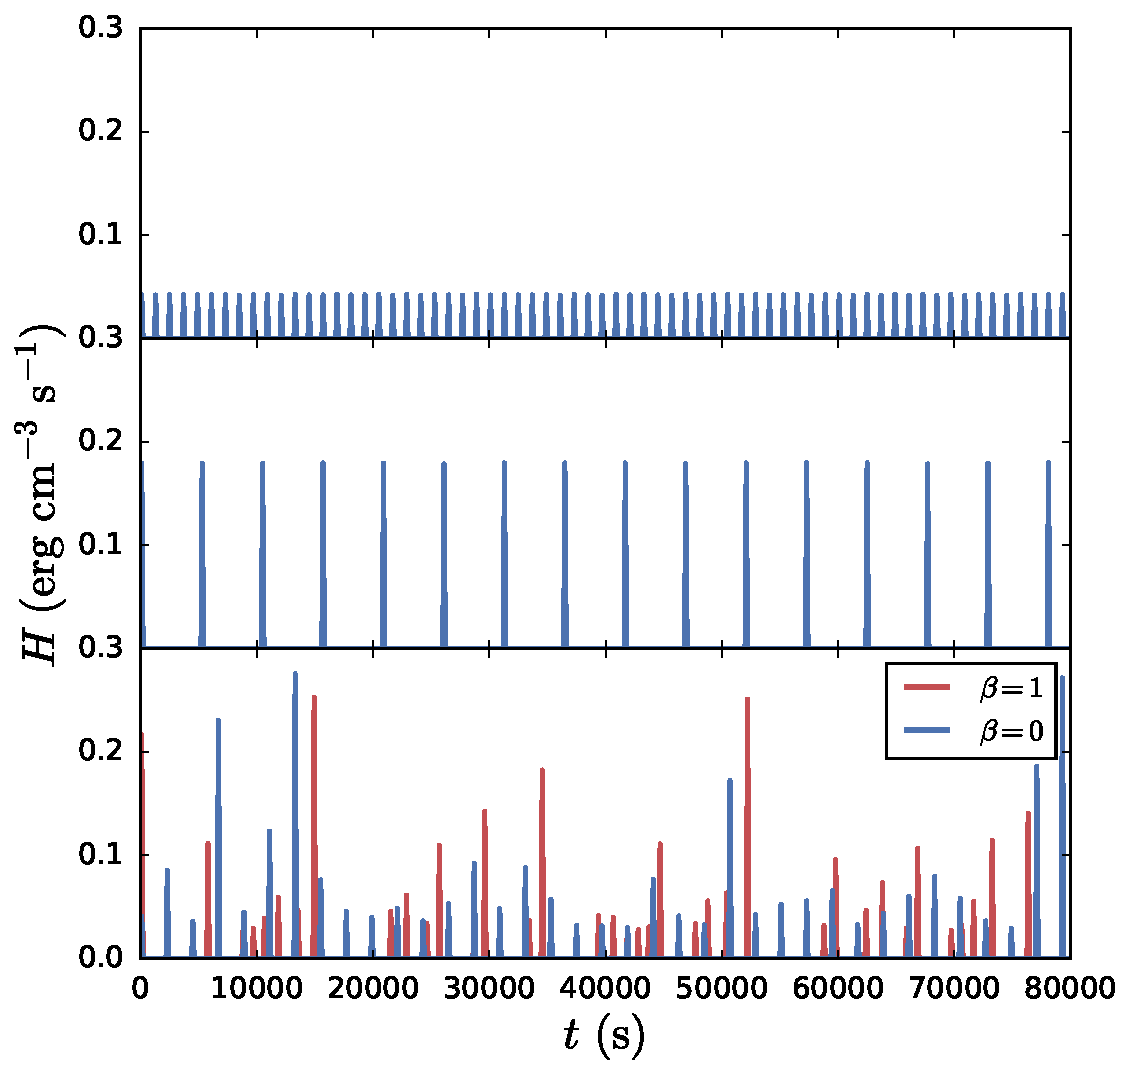
\includegraphics[width=\columnwidth]{figures/heating_functions.pdf}
		\caption{\textbf{Top}: uniform heating amplitudes for $t_N=1000$ s; \textbf{Middle:} uniform heating amplitudes for $t_N=5000$ s; \textbf{Bottom:} Heating amplitudes drawn from a power-law distribution with index $\alpha=-1.5$. The events shown in red have wait times that depend on the previous event energy while the events shown in blue have uniform wait times. The mean wait time in both cases is $\langle t_N\rangle=2000$ s.}
		\label{fig:heating_funcs}
	\end{figure}
%
	\par According to the nanoflare heating model of \citet{parker_nanoflares_1988}, turbulent loop footpoint motions twist and stress the field, leading to a buildup and subsequent release of energy. Following \citet{cargill_active_2014}, we let $\varepsilon_i\propto t_{N,i}^{\beta}$, where $\varepsilon_i,t_{N,i}$ are the total energy and waiting time following event $i$, respectively, and $\beta=1$ such that the event energy scales linearly with the waiting time. The reasoning for such an expression is as follows. Bursty, nanoflare heating is thought to arise from the stressing and subsequent relaxation of the coronal field. If a sufficient amount of energy is released into the loop, the field will need enough time to ``unravel'' and ``wind up'' again before the next event such that the subsequent waiting time is large. Conversely, if only a small amount of energy is released, the field will require a shorter unwinding time, resulting in a shorter interval between the subsequent events. Thus, this scaling provides a way to incorporate a more physically motivated heating function into a hydrodynamic model which cannot self-consistently determine the heat input based on the evolving magnetic field. \autoref{fig:heating_funcs} shows the various heating functions used for several example $t_N$ values.
	%
	\subsection{Heating Statistics}
	\label{subsec:heating_stats}
	%
	\par We compute the peak heating rate per event in two different ways: 1) the heating rate is uniform such that $H_i=H_0$ for all $i$ and 2) $H_i$ is chosen from a power-law distribution with index $\alpha$ where $\alpha=-1.5,-2.0,$ or $-2.5$. For the second case, it should be noted that, when $t_N\approx5000$ s, $N\sim16$ events, meaning the events from a single run do not accurately represent the distribution of index $\alpha$. Thus, a sufficiently large number of runs, $N_{R}$, are computed for each $t_N$ to ensure that the total number of events is $N_{tot}=N\times N_{R}\sim10^4$ such that the distribution is well-represented. \autoref{fig:parameter_space} shows the parameter space we will explore. For each set of parameters and waiting time $t_N$, we compute the resulting emission measure distribution for $N$ events in a period $t_{total}$. This procedure is repeated $N_R$ times until $N\times N_R\sim10^4$ is satisfied. Thus, when $t_N=5000$ s and $N\sim15$, $N_R=625$, meaning the model is run 625 times with a heating frequency of $t_N=5000$ s in order to properly fill out the event energy distribution.
	%
	\subsection{Non-equilibrium Ionization}
	\label{subsec:nei}
	%%
	\par When considering the role of nanoflares in the production of hot plasma in AR cores, it is important to take non-equilibrium ionization (NEI) into account \citep{bradshaw_explosive_2006,reale_nonequilibrium_2008}. In a steady heating scenario, the ionization state is an adequate measure of the electron plasma temperature. Because the heating timescale is long (effectively infinite), the ionization state has plenty of time to come into equilibrium with the electron temperature. 
	%
	\par In a nanoflare train, when the heating frequency is high, the loop is not allowed to drain or cool sufficiently between events, meaning the ionization state is kept at or near equilibrium. However, as the heating frequency decreases, the loop is allowed to cool and drain more and more during the inter-event period. If the heating occurs on a short enough timescale, the ionization state will not be able to reach equilibrium with the electron plasma before the loop undergoes rapid cooling by thermal conduction. Furthermore, if the frequency is sufficiently low so as to allow the loop to drain during the inter-event period, the ionization equilibrium timescale will increase. Thus, in the context of intermediate- to low-frequency nanoflares, NEI should be considered.
	%
	\par As in \citetalias{barnes_inference_2016}, we use the numerical code\footnote{This code has been made freely available by the author and can be downloaded at: \url{https://github.com/rice-solar-physics/IonPopSolver}.} outlined in \citet{bradshaw_numerical_2009} to compute the non-equilibrium ionization states and the corresponding effective electron temperature, $T_{eff}$ that would be inferred by assuming ionization equilibrium. Using $T_eff$, we are then able to compute a corresponding NEI emission measure distribution.
	%%
	\section{Results}
	\label{sec:results}
	%
	\par We now show the results of our loop simulations for each point in our multi-dimensional parameter space: species heated (electron or ion ), power-law index ($\alpha$), heating frequency ($t_N$), and waiting-time/event energy relationship ($\beta$). All results were processed using the IPython system for interactive scientific computing in Python \citep{perez_ipython:_2007} as well as the NumPy and Scipy numerical and scientific Python libraries \citep{van_der_walt_numpy_2011}. All results were visualized using the matplotlib graphics library \citep{hunter_matplotlib:_2007}.
	%
	\par In order to compactly summarize all of the data in each run of our model, we calculate the resulting emission measure distribution using the familiar expression $\mathrm{EM}=n^2(2L)$, where $L$ is the loop half-length. We consider a temperature range of $4.0\le\log{T}\le8.5$ with bin sizes of $\Delta\log{T}=0.01$. At each iteration $i$, the coronal temperature range $[T_0,T_a]$ is calculated from $\bar{T}_e$. For each bin that falls within $[T_0,T_a]$, $\bar{n}_i^2(2L)$ is added to that bin, where $\bar{n}_i$ is the spatially-averaged number density at time $t_i$. The emission measure in each bin is then averaged over the entire simulation period. When measured observationally, $\mathrm{EM}(T)$ is a line-of-sight quantity. Assuming an aspect ratio (i.e. ratio of loop length to loop width) of 10, we apply a correction factor 1/10 to all calculated $\mathrm{EM}$ curves. Furthermore, each emission measure distribution we also compute the corresponding effective emission measure distribution, $\mathrm{EM}(T_{eff})$, using $T_{eff}$, the effective temperature calculated by including effects due to NEI.
	%
	\par As noted in \autoref{subsec:heating_stats}, for each heating frequency $t_N$, we compute $N_R$ runs such that there are $N_R$ $\mathrm{EM}(T)$ distributions for each $t_N$. Thus, the $\mathrm{EM}(T)$ that we show for each $t_N$ is the average computed over all $N_R$ of these emission measure distributions. 
	%\par To characterize the emission measure, we compute the slopes on both the cool and hot sides of the peak. To be consistent with past observational and computational studies of cool emission \citep[see][and references therein]{bradshaw_diagnosing_2012}, we fit the cool slope on the interval $6.0\le\log{T}\le6.6$. Contrastingly, past studies of hot emission are less abundant; thus, the ``hot'' region where the $\mathrm{EM}$ is thought to follow a power-law is far less constrained. In order to best describe the steepness of the emission measure hotward of the peak, we choose to fit $\mathrm{EM}$ between the temperatures at which the emission measure is $99\%$ and $92\%$ of the peak value. We have no physical reason for choosing these particular bounds, but note that on this interval, the mean hotward emission is reasonably well-described by a power-law relationship. Fitting too close to the wide peak leads to misleadingly shallow slopes while fitting too close to the steep drop near $\log{T}\sim7.5$ results in steep slopes not particularly representative of the hotward emission. We perform the fit using the Levenberg-Marquardt algorithm for least-squares curve fitting as implemented in the SciPy scientific Python package \citep{van_der_walt_numpy_2011}.
	%
	\subsection{Emission Measure Distributions}
	\label{subsec:em_dist}
	%
	\begin{figure*}[t]
		\centering
		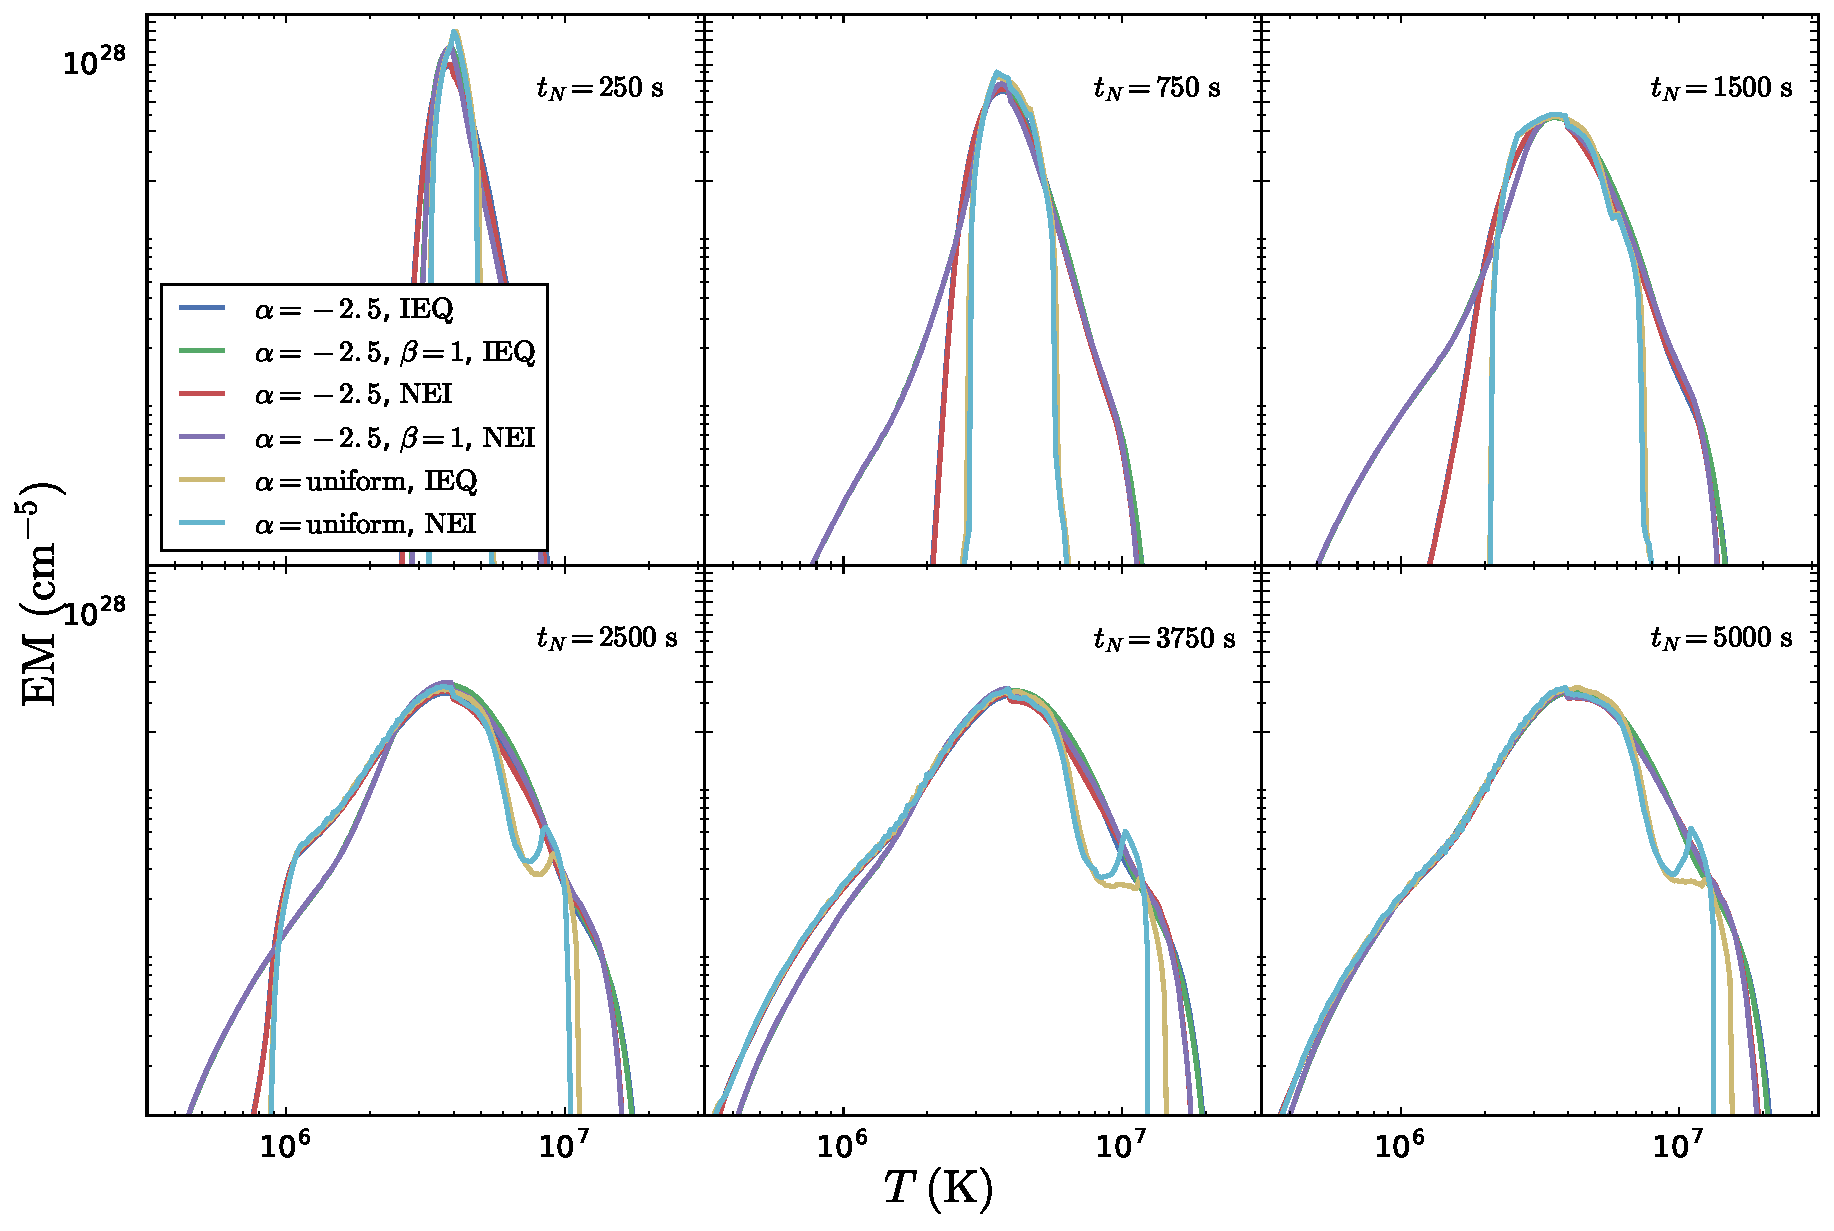
\includegraphics[width=2\columnwidth]{figures/em_grid_electron_a25.pdf}
		\caption{Emission measure distributions for varying waiting-times, $t_N$ in the case where only the electrons are heated. The three types of heating functions shown are uniform heating rates (red), heating rates chosen from a power-law distribution of $\alpha=-2.5$ (blue), and heating rates chosen from a power-law distribution of $\alpha=-2.5$ where the time between successive events is proportional to the heating rate of the preceding event (green). The dotted lines denote the corresponding $\mathrm{EM}(T_{eff})$ distribution.}
		\label{fig:el_em}
	\end{figure*}
	%
	\par First, we look at the resulting emission measure distributions for the case in which only the electrons are heated. \autoref{fig:el_em} shows $\mathrm{EM}(T)$ for six different values of $t_N$ and three different types of heating functions: uniform heating events, events chosen from a power-law distribution of index $\alpha=-2.5$, and events chosen from a power-law distribution of index $\alpha=-2.5$ where the time between successive events depends on the heating rate of the preceding event. The dotted lines in each frame show the corresponding emission measure distribution constructed from $T_{eff}$, $\mathrm{EM}(T_{eff})$.
	%
	\par As $t_N$ increases, $\mathrm{EM}$ is allowed to extend to both lower and 
	%
	\begin{figure*}
		\centering
		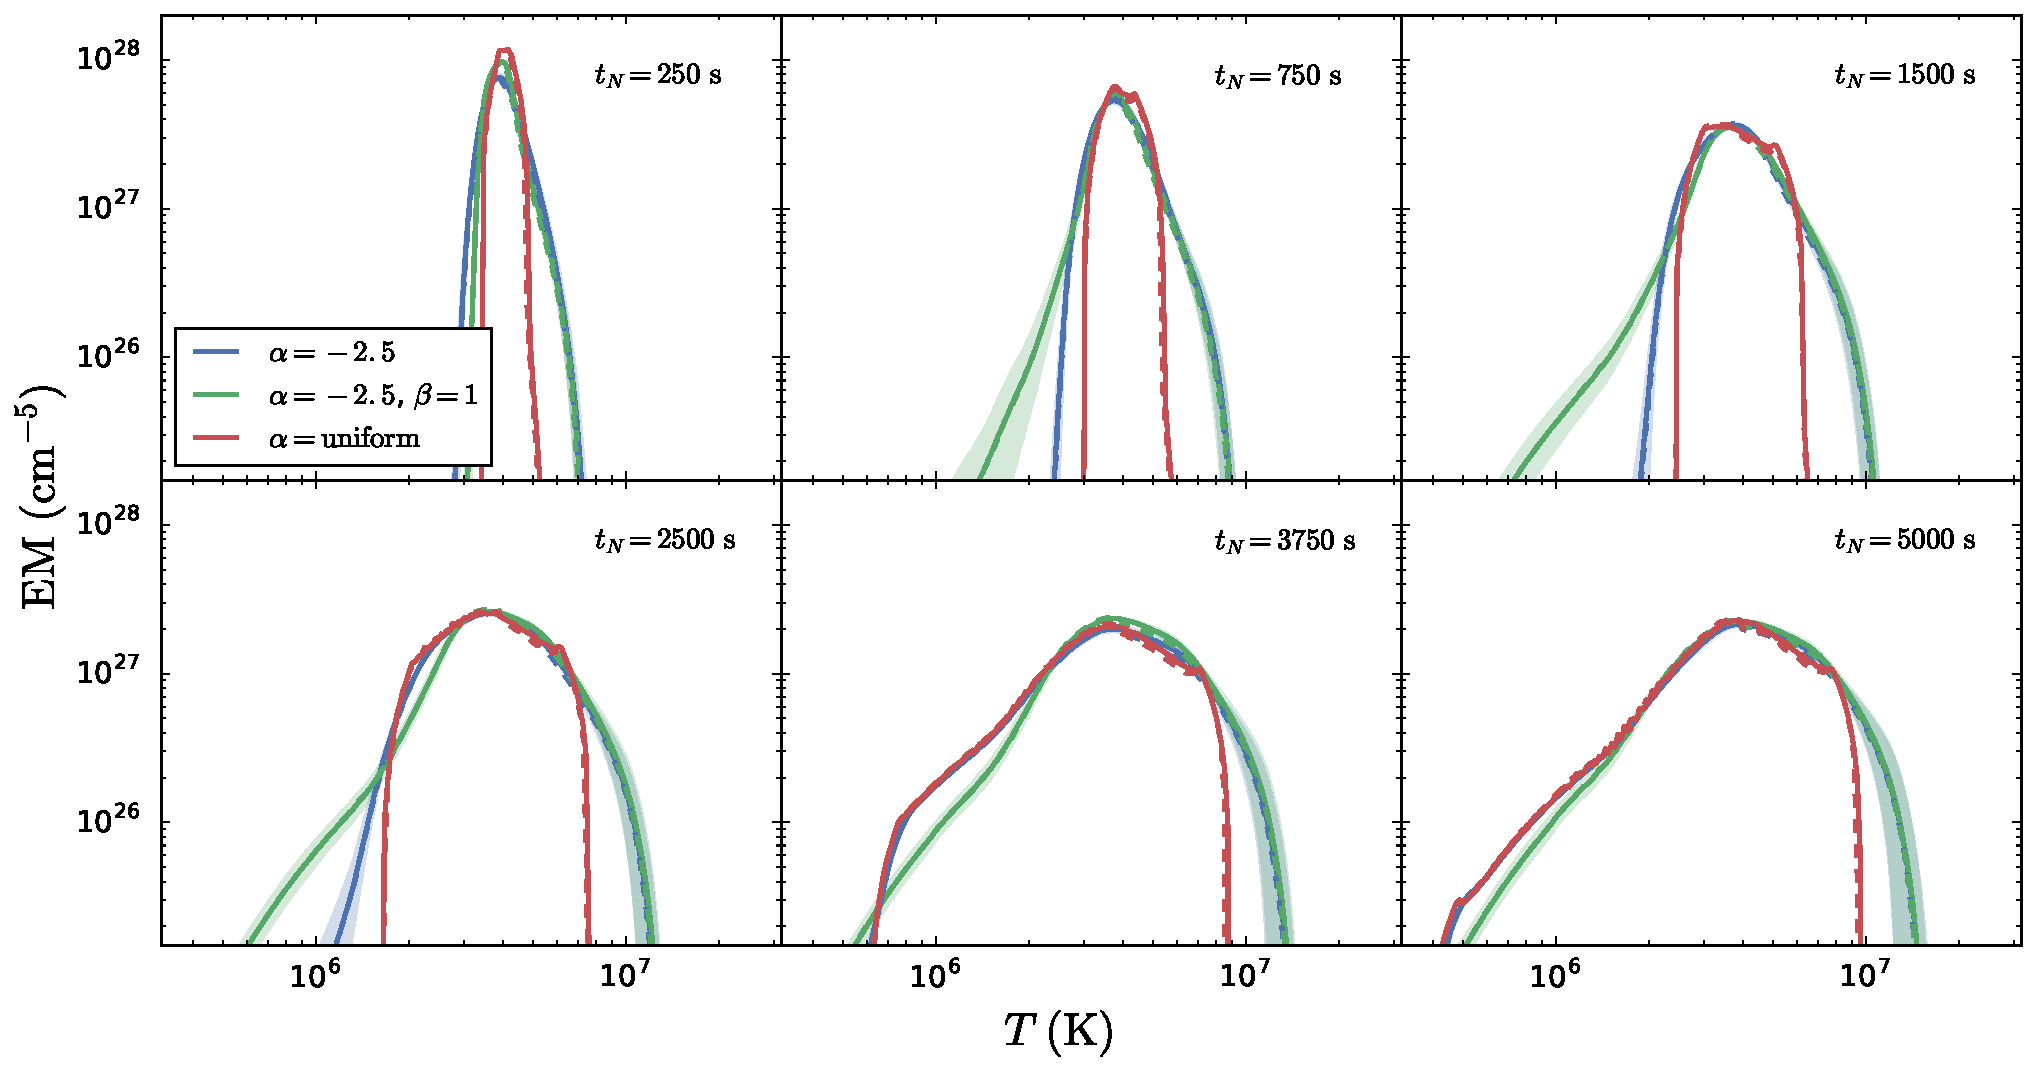
\includegraphics[width=2\columnwidth]{figures/em_grid_ion_a25.pdf}
		\caption{Same as \autoref{fig:el_em}, but for the case where only the ions are heated.}
		\label{fig:ion_em}
	\end{figure*}
	%
	\par \autoref{fig:el_em} and \autoref{fig:ion_em} show the results of our emission measure study for the two distinct cases where only the electrons are heated and only the ions are heated with $\alpha=-2.5,\beta=1$ for a loop half-length of $40$ Mm, consistent with \citetalias{barnes_inference_2016}. The panels on the left show the mean $\mathrm{EM}$ for all $t_N$, where the average is taken over all $N_{R}$ runs. There is an artifical spacing of $\Delta\log{\mathrm{EM}}=0.2$ between each curve so that they can be easily distinguished from each other. The blue (red) lines indicate the cool (hot) power-law fits, where the slopes of the lines are the averages taken over all $N_{R}$ runs. We note that the $\mathrm{EM}$, for all $t_N$, peaks at approximately 4 MK ($10^{6.6}$ K), consistent with the constraints laid out in \autoref{subsec:params}. The top right panels show these average slope values as a function of $t_N$. The error bars indicate one standard deviation as calculated from the distribution of all $N_{R}$ runs.
	%
	\par Lastly, the bottom right panels show the first derivative as a function of temperature, $d\log{\mathrm{EM}}/d\log{T}$, computed using central differences. The color scheme and line styles correspond to the emission mesure curves in the left panel. As in \citetalias{barnes_inference_2016}, we compute the derivative in an effort to better assess at what temperatures the emission measure is not well described by a power-law.
	%
	\par We first briefly consider the calculated cool emission measure slopes. Looking at the top right panels of \autoref{fig:el_em} and \autoref{fig:ion_em}, we note that in the cases of electron and ion heating, the cool emission measure slopes are consistent with both observational and modeling studies of cool emission in AR cores, having values that fall within the range $2\le a\le5$ \citep[and references therein]{bradshaw_diagnosing_2012}. Furthermore, the cool slopes computed using our new modified EBTEL model, with a heating function of the form $Q\propto T_N^{\beta}$, are consistent with those values reported in \citet{cargill_active_2014} and show a dependence on the waiting time $t_N$.  
	%
	\par Additionally, looking at the bottom right panels of \autoref{fig:el_em} and \autoref{fig:ion_em}, we see that, within the range $6.0\le\log{T}\le6.6$, the $\mathrm{EM}$ is reasonably well-described by a power-law, where $2\lesssim d\log{\mathrm{EM}/d\log{T}}\lesssim3$. Comparing the cases of electron and ion heating for both the cool slopes and $d\log{\mathrm{EM}/d\log{T}}$ on $6.0\le\log{T}\le6.6$, there are no substantial differences for all values of $t_N$ considered.
	%
	\par This is not the case for the hot emission measure. Looking first at the case of electron heating in \autoref{fig:el_em}, we note that there is a pronounced ``hot shoulder'' in the emission measure (left panel) just above $10^7$ K for $T_N\gtrsim2000$ s. This feature is even more evident when looking at the derivative of $\mathrm{EM}$ in the bottom right panel of \autoref{fig:el_em}. The peak between $10^7$ and $10^{7.5}$ K shows how the $\mathrm{EM}$ flattens out around $10^7$ K, indicating an enhanced hot emission measure. Considering the large range of values of $d\log{\mathrm{EM}}/d\log{T}$ on the interval over which the fit was performed, we acknowledge that a single power-law fit is not a good description of the hot emission measure in the case of electron heating.
	%
	\par Contrastingly, we have not calculated the hot emission measure slopes for the case of ion heating. Looking at the left panel of \autoref{fig:ion_em}, for $T_N\gtrsim1000$ s, the $\mathrm{EM}$ peak is wide with a sharp cutoff just above $10^7$ K. There is no substantial emission measure component above $10^7$ K and, consequently, no hot shoulder as in the electron heating case. Applying the fitting procedure outlined above to the hot emission in the case of ion heating yields meaningful results for only a few short $t_N$. Thus, as in the case of electron heating, the resulting hot emission measure from ion heating is also not well described by a power-law. The lower right panel of \autoref{fig:ion_em} further highlights this by showing that around $10^7$ K, $d\log{\mathrm{EM}}/d\log{T}\to-\infty$.
	%
	\subsection{Pre-nanoflare Density}
	\label{subsec:pre_nanoflare_density}
	%
	\begin{figure*}
		\centering
		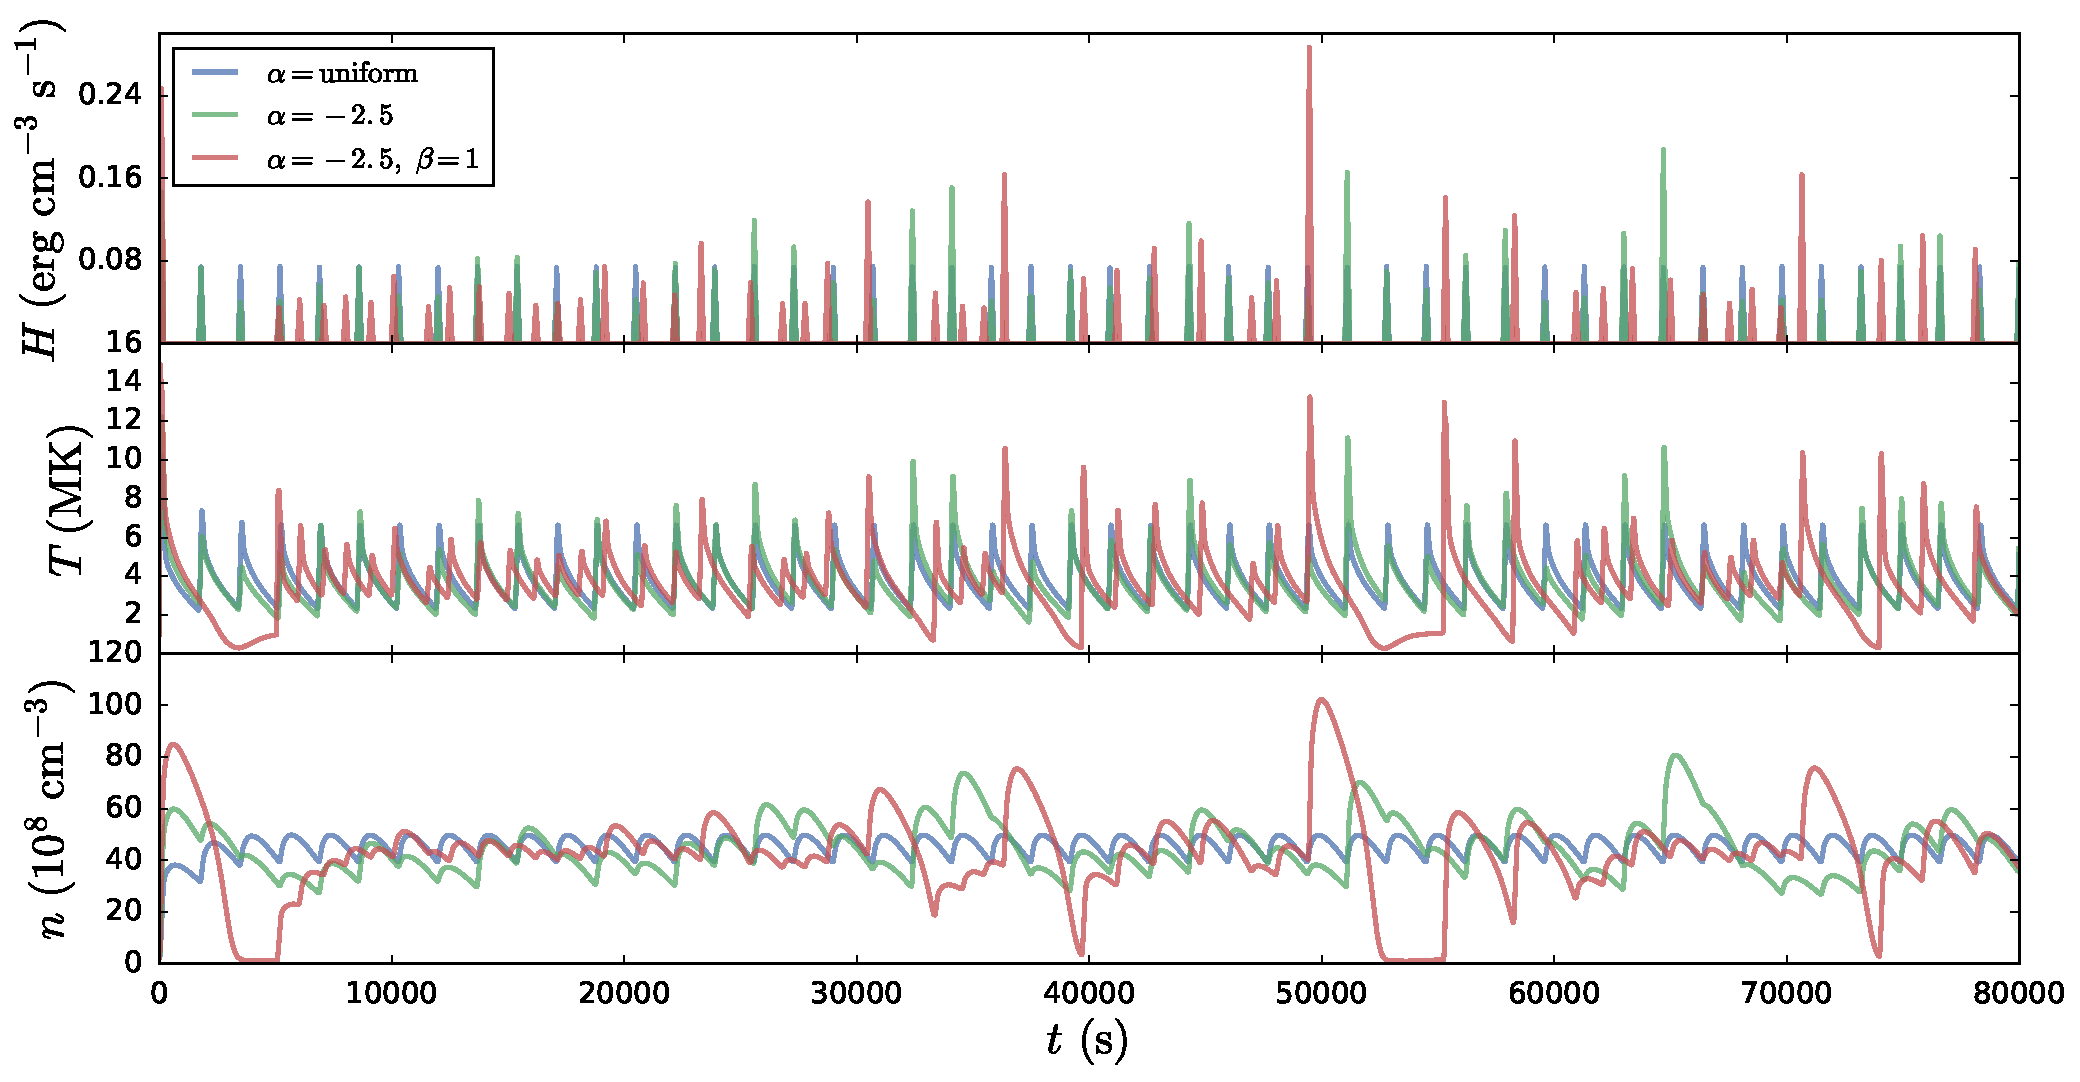
\includegraphics[width=2\columnwidth]{figures/nT_sample_curves_tn1500_electron.pdf}
		\caption{Example temperature and density profiles for an intermediate heating frequency, $t_N=1500$ s for several different heating function types.}
	\end{figure*}
	%
	\par \autoref{fig:single_em} shows the same results as \autoref{fig:el_em} and \autoref{fig:ion_em}, but for the single-fluid case in which electron-ion equilibrium is assumed at all times. To compute these $\mathrm{EM}$ curves, we have used the original, single-fluid EBTEL model as described in \citet{klimchuk_highly_2008} and \citet{cargill_enthalpy-based_2012}. The equivalent parameter space that was investigated with the modified two-fluid EBTEL model is explored with the single-fluid EBTEL code as well.
	%
	\par We compute the hot and cool emission measure slopes in the same manner as the electron and ion heating cases. We first note that the cool emission measure slopes are comparable to those in both the electron and ion heating cases. In particular, we find $2\lesssim a\lesssim5$ for all values of $t_N$ as expected. Again, we confirm the validity of our linear fit to the cool emission by computing the derivative $d\log{\mathrm{EM}}/d\log{T}$ in the lower right panel of \autoref{fig:single_em}. For $T_N\gtrsim2000$ s, the slope is bounded between 2 and 3 on the interval $6.0\le\log{T}\le6.6$. 
	%
	\par The hot emission measure in the single-fluid case differs significantly from the two-fluid case. In contrast to the electron heating case in \autoref{fig:el_em}, the $\mathrm{EM}$ curves in the left panel of \autoref{fig:single_em} show no hot shoulder. This is further confirmed by the lower right panel; the derivative, in contrast to the electron heating case, shows no peak near $10^7$ K. For low $t_N$, $d\log{\mathrm{EM}}/d\log{T}$ is monotonically decreasing for $\log{T}\gtrsim6.6$. For $T_N\ge3000$ s, $d\log{\mathrm{EM}}/d\log{T}$ is relatively flat for $\log{T}\ge7.0$, indicating that a power-law provides a good description of the hot emission in this region. This is confirmed by noting the agreement between the fit lines and the $\mathrm{EM}$ curves in the left panel.
	%
	\par Comparing the top right panels of \autoref{fig:single_em} and \autoref{fig:el_em} further highlights the enhanced hot emission in the electron case. For high $t_N$, the hot emission slopes in the electron case converge to a value just above 3; for the single-fluid case, the hot slopes converge to approximately 4.5. Thus, while a single power-law is not a good descriptor for the hot emission in the case of electron heating, the slope still captures the enhanced hot shoulder relative to the weaker hot emission of the single-fluid case. Additionally, comparing the single-fluid case to the ion heating case in \autoref{fig:ion_em}, it is obvious that the single-fluid case shows a great deal more hot emission as the $\mathrm{EM}$ curves in the left panel of \autoref{fig:single_em} extend well above $10^7$ K while those in the left panel of \autoref{fig:ion_em} show a steep cutoff at temperatures just above the peak.
	%
	\subsection{Hot Plasma Diagnostics}
	\label{subsec:diagnostics}
	%%
	\begin{figure*}
		\centering
		\subfigure[]{%
		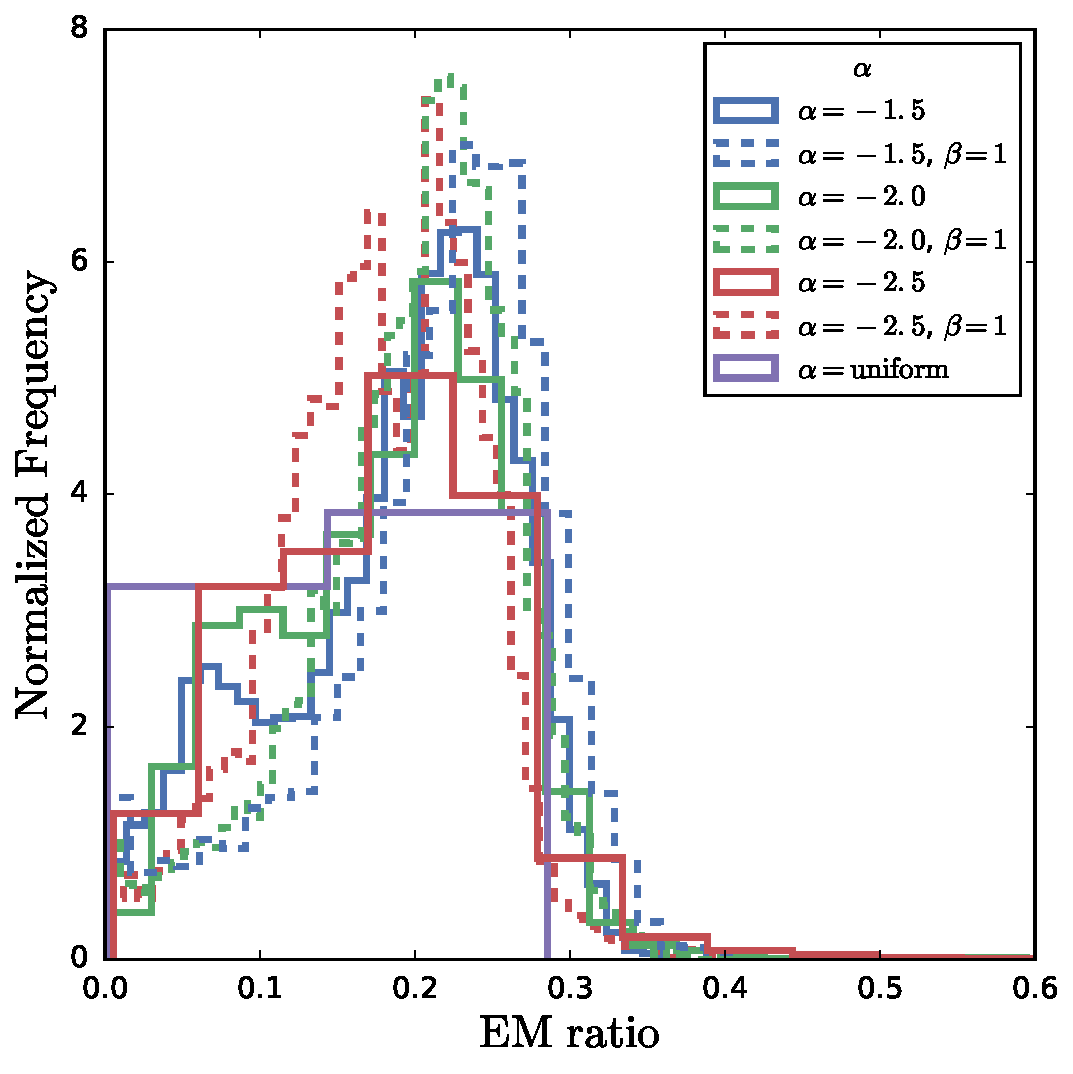
\includegraphics[width=\columnwidth]{figures/ratio_hist_alpha_electron_T0.pdf}
		}
		\subfigure[]{%
		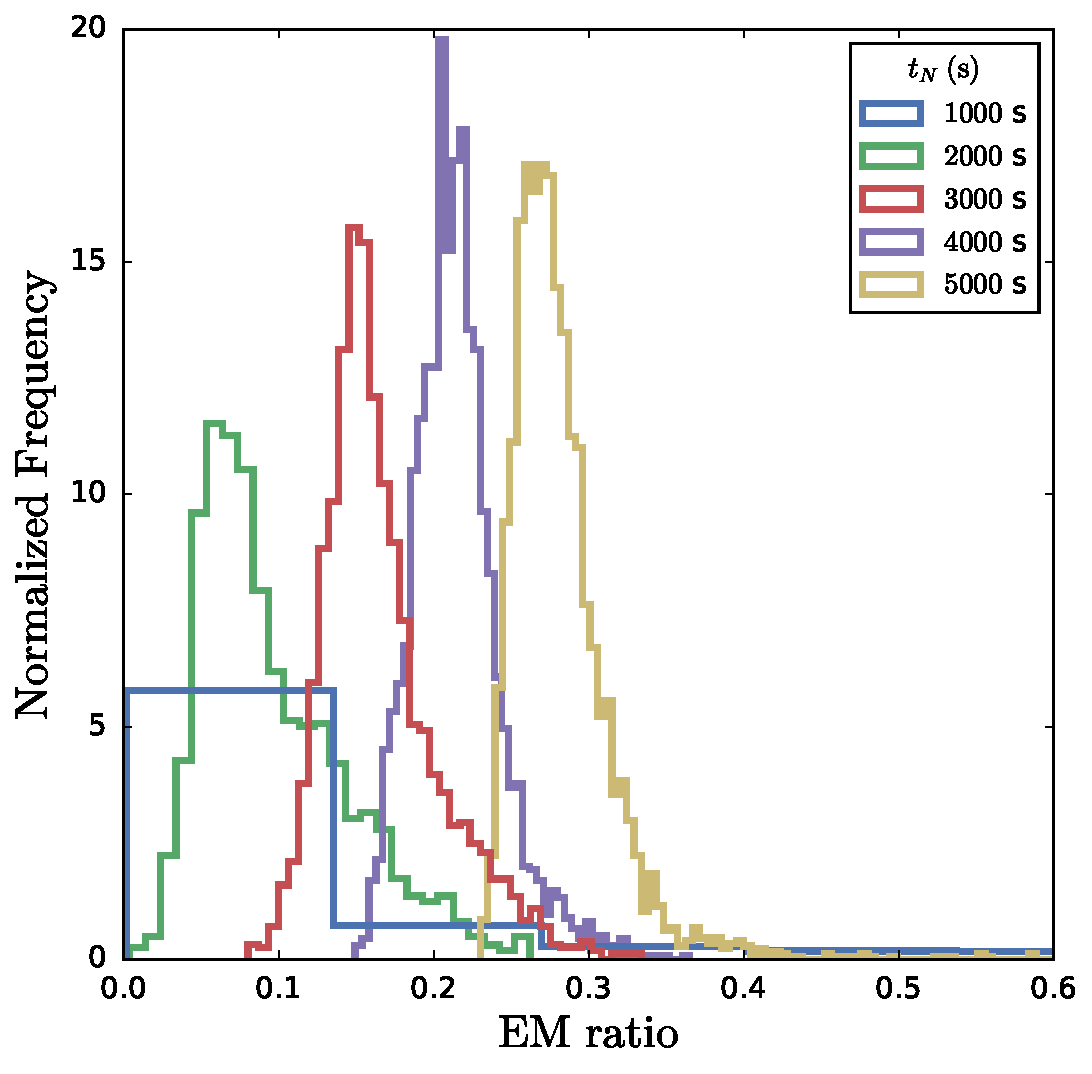
\includegraphics[width=\columnwidth]{figures/ratio_hist_twait_electron_T0.pdf}
		}
		\caption{Electron heating emission measure ratio for an EIS/MaGIXS line pair}
	\end{figure*}
	%%
	\begin{figure*}
		\centering
		\subfigure[]{%
		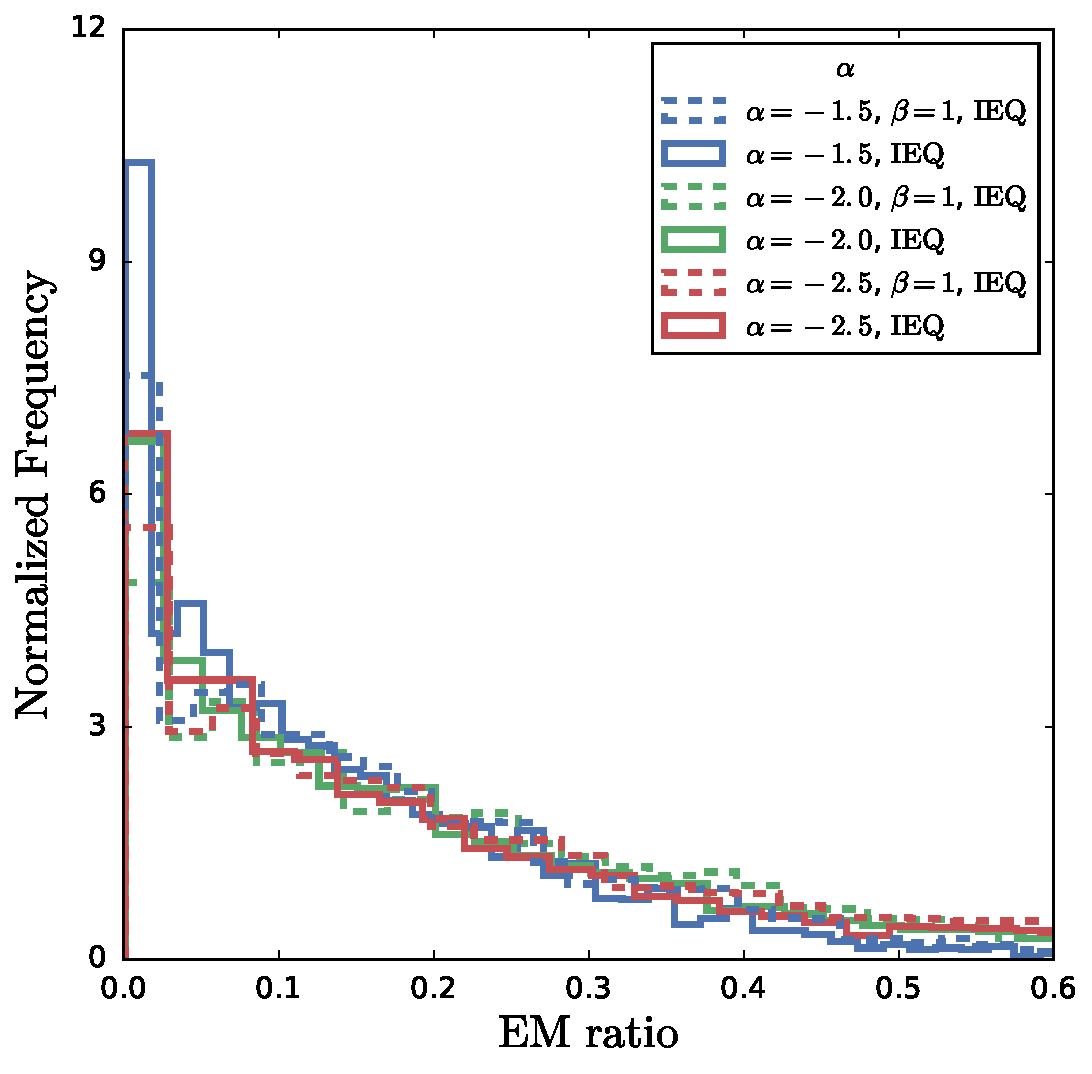
\includegraphics[width=\columnwidth]{figures/ratio_hist_alpha_ion_T0.pdf}
		}
		\subfigure[]{%
		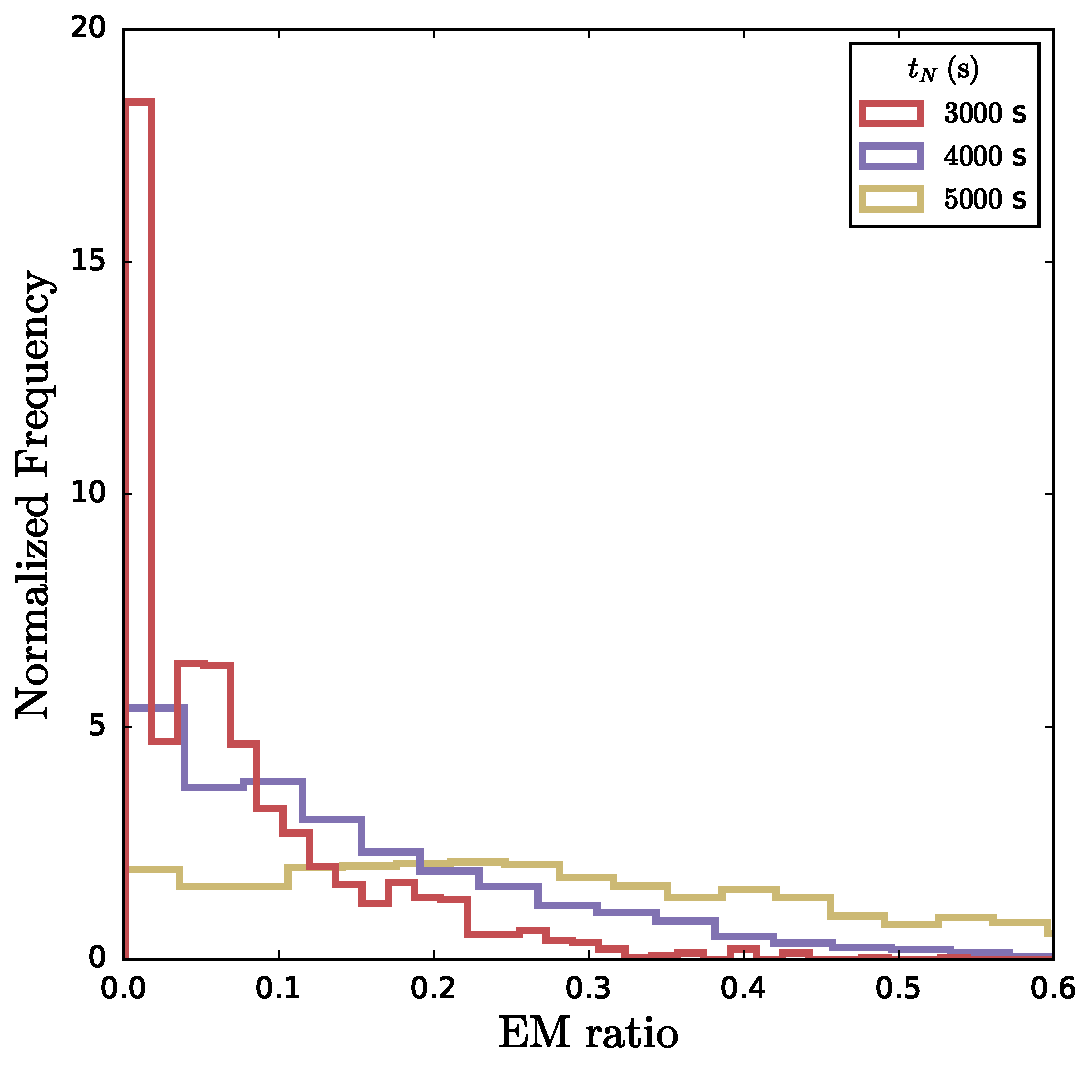
\includegraphics[width=\columnwidth]{figures/ratio_hist_twait_ion_T0.pdf}
		}
		\caption{Diagnostics figures}
	\end{figure*}
	%%
	\par As mentioned in \autoref{sec:intro}, NEI can make it difficult to observe emission signatures from nanoflare-heated plasma because the heating timescale is shorter than the ionization timescale such that the charge state of the plasma is not representative of the plasma temperature. In order to diagnose how NEI might affect hot emission measure slopes, we use $n$ and $T_e$ profiles from our modified EBTEL code along with the method outlined by \citet{bradshaw_numerical_2009} to compute $T_{eff}$, the temperature that would be measured based on the actual ionization states. An effective emission measure distribution, $\mathrm{EM}_{eff}$, can then be calculated. Following \citetalias{barnes_inference_2016}, we use iron (Fe) and the ionization states Fe IX through FeXXV.
	%
	\par As the calculation of $T_{eff}$ is significantly more expensive than an EBTEL calculation, we do not compute $\mathrm{EM}_{eff}$ for the entire parameter space and instead consider only a small number of single-pulse test cases of duration $\tau_H=100$ s and peak heating rate $H_0=0.8$ erg cm$^{-3}$ s$^{-1}$. \autoref{fig:teff_test_case} shows temperature and density profiles (left column)  and emission measure distributions (right column) for the cases where NEI is (dashed) and is not (solid) included. These profiles are computed for all preferentially-heated species (electron, ion, single-fluid). For all three species, we note that including NEI in the calculation of the cool slope makes essentially no difference .
	%
	\par As in \autoref{fig:ion_em}, we do not compute the hot slope for the case of ion heating. Looking at the right panel in the middle row of \autoref{fig:teff_test_case}, we see that the inclusion of NEI in the case of ion heating has little to no effect on the emission measure. This is confirmed by the left panel of the middle row which shows that the difference between $T$ and $T_{eff}$ is relatively small and only occurs at low densities. Conversely, in the single-fluid and electron-heating cases, $T$ and $T_{eff}$ differ greatly during the heating phase and NEI has two distinct effects on the $\mathrm{EM}$: it leads to an overestimation of the amount of emission in the mid-range hot temperatures ($7.0\lesssim\log{T}\lesssim7.2$) and causes a steeper cutoff in the emission at lower temperatures (before $\log{T}\approx7.25$) compared to the case where NEI is not included. Interestingly, in both the electron-heating (first row) and single-fluid (third row) cases, $b_{eff}<b$ though we note that in the electron-heating case (first row), a power-law fit does not adequately describe the hot side of the $\mathrm{EM}$ distribution.
	%
	\par To compare the effects of varying $\alpha$, $\beta$, and $t_N$ for each species (i.e. electron, ion, single-fluid), we construct histograms of hot and cool emission measure slopes for each parameter space point. Recall that in the case where the distributions of heating event energies are non-uniform, we have $N_{R}$ emission measure slopes to properly account for the statistical spread in hot emission measure slopes due to power-law distributions.
	%
	\par As seen in \autoref{fig:histos}, these histograms, denoted by type of slope (i.e. hot or cool) and species, are constructed in one of two ways: each distinct histogram (denoted by linestyle and/or color) is either representative of a distinct heating function (e.g. top row of \autoref{fig:histos}) or a distinct value of $t_N$ (e.g. bottom row of \autoref{fig:histos}). In the four panels of \autoref{fig:histos}, we choose to separate the cool emission measure slopes by type of heating function and the hot emission measure slopes by $t_N$. This means, for example, that the dot-dashed blue $\alpha=-1.5,\beta=1$ histogram in the upper left panel of \autoref{fig:histos} encapsulates cool emission measure slopes for $250\le T_N\le5000$ s while the solid blue $T_N=2000$ s histogram in the lower left panel includes emission measure slopes for all 10 types of heating functions (as listed in \autoref{fig:parameter_space} and the legend in the upper left panel of \autoref{fig:histos}). All histograms are normalized such that for each distribution $P(x)$, $\int_{-\infty}^{\infty}\mathrm{d}x~P(x)=1$. Additionally, the bin widths are calculated using the well-known Freedman-Diaconis formula \citep{freedman_histogram_1981}.
	%
	\par Concerning the distributions of cool slopes grouped by type of heating function (bottom row of \autoref{fig:histos}), we note that there are no discernible differences between the cases of electron and ion heating. In both cases, all heating functions except for those where $\beta=1$ are peaked sharply between 2 and 2.5. In the case where $\beta=1$ (for all $\alpha$), the distribution is peaked between 2.5 and 3, with the width of the distribution increasing as $\alpha$ steepens. This larger range of cool emission measure slopes for the case of $\beta=1$ is consistent with \citet{cargill_active_2014}.
	%
	\par As stated in \autoref{subsec:electron_ion_heating}, we choose not to show the hot emission measure slopes for the ion heating case as they are not representative of the emission measure distribution hotward of the peak as evidenced by the left and bottom right panels of \autoref{fig:ion_em}. Instead, we compare the hot emission measure slopes of the electron heating and single-fluid cases, the bottom left and bottom right panels of \autoref{fig:histos}, respectively. In both cases, for $T_N<3000$ s, we see a strong dependence on $t_N$ while for $T_N\ge3000$ s, the slopes tend to be sharply peaked around a single value. In the electron heating case, distributions for $T_N<3000$ s tend to be more narrow than their single-fluid counterparts and centered at lower values (i.e. more shallow hot slopes). Most notably, for $T_N\ge4000$ s, the electron heating hot emission measure slopes are peaked between 3 and 3.5 while the single-fluid slopes are peaked at $\sim4.5$. 
	%
	\section{Discussion}
	\label{sec:discussion}
	%
	\par The main points we emphasize from the results presented in \autoref{sec:results} are,
	\begin{enumerate}
		\item Cool emission measure slopes resulting from electron and ion heating are very similar and are well described by $\mathrm{EM}\propto T^a$. As noted in \citet{cargill_active_2014}, using the relation $Q\propto T_N^{\beta}$ yields $2\lesssim a\lesssim5$, consistent with observations.\label{itm:cool}
		\item Hot emission from electron heating results in an enhanced hot shoulder while the equivalent ion heating cases show a relatively flat peak and a steep dropoff near $10^7$ K. This effect is exacerbated as $t_N$ increases.\label{itm:hot}
		\item Hot emission due to both electron and ion heating is poorly described by the scaling $\mathrm{EM}\propto T^{-b}$. In the former, this is due to the flat hot shoulder between $10^7$ and $10^{7.5}$ K. In the latter case, the relatively flat peak and steep drop off near $10^7$ K do not allow for a power-law description of the hot emission.\label{itm:deriv}
		\item Using a power-law to describe the hot side of the $\mathrm{EM}$ distribution, single-fluid models predict less hot-emission than two-fluid models in which only the electrons are heated. In particular, for $T_N\ge4000$ s, our modified two-fluid EBTEL model predicts $3\le b\le3.5$ while the original single-fluid EBTEL model predicts $b\sim4.5$.\label{itm:histos}
		\item Including NEI does not impact the cool emission measure slope. In the case of electron heating and the single-fluid case, NEI enhances the mid-range hot $\mathrm{EM}$, but leads to a lower temperature cutoff. The emission measure distribution in the case of ion heating is unaffected. \label{itm:nei}
	\end{enumerate}
	%
	\par We first focus on \autoref{itm:cool}. In the range $6.0\le\log{T}\le6.6$, the loop is undergoing both radiative and enthalpy-driven cooling. During this phase, the density is high and the temperature low relative to the heating and conductive cooling phase. Looking at the fourth term on the right-hand side of \autoref{eq:press_e} and \autoref{eq:col_freq}, the coupling term between the two species is roughly $\propto\bar{n}^2(\bar{T}_e-\bar{T}_i)/\bar{T}_e^{3/2}$; as density increases, so does the coupling strength. While the loop is also draining in this temperature range, the density has already increased such that $\bar{T}_e\approx\bar{T}_i$ and until the next heating event, there is nothing to drive the two species out of equilibrium. Thus, because the two-species are evolving together in this regime, we expect their emission measure distributions to be the same.
	%
	\par In \autoref{itm:hot}, we see quite the opposite situation. In the heating and conductive cooling phases, the density is relatively low and the electron (or ion) temperature relatively high. Because the heating pulses we have used are relatively short (100 s), the heated species quickly reaches high temperatures and cools significantly by thermal conduction before Coulomb collisions can bring the two species back into equilibrium. Since the emission measure depends on the electron temperature, this means that in the event that only the electrons are heated, the emission  ``sees'' the full range of temperatures produced by heating and conductive cooling.
	%
	\par However, in the case of ion heating, in order for the emission measure to see the full range of temperatures resulting from the heating and conductive cooling by the ions, $\bar{T}_e=\bar{T}_i$ would have to hold for this entire phase. Instead, as the ions are impulsively heated, the electrons remain at a relatively low temperature, coupled only weakly to the ions because the loop has only just begun to fill. As the coronal density increases, the electrons come into equilibrium with the ions, but because thermal conduction is such an efficient cooling mechanism in the corona, the ions have now cooled far below the temperature to which they were initially heated. 
	\par The result is a severely truncated hot emission measure distribution as seen in \autoref{fig:ion_em}. Additionally, this effect is exacerbated at long $t_N$. For short $t_N$, the heating is essentially steady, meaning that the loop has little to no time to drain or cool between heating events. This keeps the density at a roughly constant, near-equilibrium value which inhibits rapid heating to high temperatures and keeps the electrons and ions in equilibrium. However, for longer $t_N$, the loop is allowed to drain significantly between each pulse. Thus, at the start of each heating event, the density is low, allowing the species to very quickly evolve out of equilibrium. 
	%
	\par Finally, \autoref{itm:nei} addresses the fact that NEI does not affect cool emission or emission due to ion heating, while it acts to enhance mid-range hot temperature emission and creates a lower-temperature cutoff in the single-fluid and electron heating cases as shown in \autoref{fig:teff_test_case}. As discussed in \citetalias{barnes_inference_2016} and \autoref{sec:intro}, if the heating occurs on a timescale faster than the ionization equilibration timescale, high temperatures will not be detectable because the charge states indicative of such temperatures will not have had time to form. Coolward emission is due to radiative and enthalpy-driven cooling and during this phase, the density is relatively high and the temperature is changing relatively slowly, meaning that ionization equilibrium can be assumed. 
	\par For hotward emission in the case of ion heating, we note that the effective heating timescale for the electrons is approximately $\tau_{ei}$, the coupling timescale. For $Q\approx10^{25}$ erg, the electron temperature increases relatively slowly (compared to the heating timescale of the ions) and only gets above several MK once the density has increased significantly. Thus, ionization equilibrium can be assumed because the electrons undergo no direct impulsive heating. In the cases of electron heating and the single-fluid case, the electrons undergo direct impulsive heating when the density is relatively low. This is what leads to the lower-temperature cutoff in $EM_{eff}$: at these high temperatures and low densities, the ionization equilibration timescale is significantly longer than the heating timescale and so these very high temperatures are never seen. 
	%
	\par However, looking at the left panels in the first and third rows of \autoref{fig:teff_test_case}, we see that just after the heating ends at 100 s, $T_{eff}>T$ due to the fact that the thermal conduction timescale is shorter than the ionization equilibration timescale. This lag in the charge state due to the efficiency of thermal conduction leads to the mid-range hot temperature emission enhancement seen in the right panels of the first and third rows of \autoref{fig:teff_test_case}. 
	%
	\section{Conclusions}
	\label{sec:conclusions}
	%
	\par In this paper, we have used a modified two-fluid version of the popular EBTEL model to study the effect of preferentially heating the electrons or ions on the hot and cool emission measure slopes over a parameter space that includes the power-law index describing the distribution of event energies, $\alpha$, waiting time between successive heating events, $t_N$, and the scaling between the event energy and wait time, $\beta$. We have found that while there is little difference in the cool emission between the cases of electron and ion heating, the emission measure curves of the electron-heated loops have an enhanced hot shoulder due to faster loop filling times and steepened hot mid-range slope due to accelerated cooling by the Coulomb collisions while the ion-heated loops show a truncated emission measure distribution on the hot side. These differences become more prominent as $t_N$ increases. We note that given such a distinction in the $\mathrm{EM}$ distribution between the cases of electron and ion heating, the difference could be potentially observationally diagnosable by instruments such as MaGIXS, the Focusing Optics X-ray Solar Imager (FOXSI) \citep{krucker_focusing_2011}, or other future missions with adequate spectroscopic resolution in the hard X-rays.
	\par Furthermore, by comparing these results with emission measure distributions obtained from the original single-fluid EBTEL model, we have found that heating only the electrons and using a single power-law fit leads to significantly smaller hot emission measure slopes for equivalent values of $t_N$. Thus, using a single-fluid model to interpret observed hot emission measure distributions can potentially lead to a misdiagnosis of the heating frequency. Additionally, characterizing the hotward emission with a single power-law fit, as is common practice with cool emission, does not adequately capture all of the features of the hotward emission.
	%
	\par We note that in this study, we have constructed the most ideal emission measure curves by using the expression $\mathrm{EM}=n^2(2L)$; that is, we have not taken into account the many complications involved when computing emission measure distributions from observed spectral lines. For example, as we noted in \citetalias{barnes_inference_2016}, impulsive heating leads to NEI and a consequently lower effective temperature, meaning that the emission does not see the hottest temperatures during the conductive cooling phase. By computing test cases for electron heating, ion heating, and the single-fluid case, we have shown that NEI has the effect of steepening the hot emission measure distribution at very high temperatures and enhancing the mid-range hot temperature emission for the electron heating and single-fluid cases, but has no impact on the emission measure distribution in the case of ion heating. We stress that when interpreting observed hot emission in the context of simulation, two-fluid and non-equilibrium ionization effects should be properly taken into account in order to extract meaningful properties of the heating.
	%
	\section*{Acknowledgment}
	%
	\hl{Acknowledge some things here.} 
	%
	%
	%Bibliography
	\bibliography{astrophys-abbrev.bib,references.bib}
	\bibliographystyle{apj}
	\clearpage
\end{document}